%%%%%%%% ICML 2025-STYLED PUBLIC REPORT %%%%%%%%%%%%%%%%%

\documentclass{article}

\usepackage{microtype}
\usepackage{graphicx}
\usepackage{booktabs}
\usepackage{amsmath}
\usepackage{amssymb}
\usepackage[accepted,nohyperref]{icml2025}

\renewcommand{\ttdefault}{cmtt}
\emergencystretch=2em
\icmltitlerunning{Can a VLM Learn to Imagine FrozenLake?}

\newcommand{\code}[1]{\texttt{#1}}
\newcommand{\todo}[1]{\textcolor{red}{#1}}

\begin{document}

\twocolumn[
\thispagestyle{plain}
\begin{center}
\rule{\textwidth}{0.8pt}
\vskip 0.24in
{\Large\bfseries Can a VLM Learn to Imagine FrozenLake?\par}
\vskip 0.20in
{\normalsize Research in LLMs, HSE $\times$ Central University\par}
\vskip 0.25in
\rule{\textwidth}{0.8pt}
\vskip 0.22in
{\bfseries Ivan A. Novosad\par}
{\ttfamily inovosad@hse.ru\par}
\vskip 0.18in
\end{center}
]

\begin{abstract}
probably yes.\textsuperscript{*}
\end{abstract}
\AddToShipoutPictureFG*{%
  \AtPageLowerLeft{%
    \put(\LenToUnit{1in},\LenToUnit{0.45in}){%
      \parbox{\textwidth}{\footnotesize\textsuperscript{*} source of well-known anecdote: \url{https://arxiv.org/abs/1110.2832}}%
    }%
  }%
}

\section{The Bet}

The assignment asks a clean question: can a VLM ``imagine'' the next transition, and can code use that transition for planning?

There are two different jobs here. A reactive VLM policy sees an image and directly chooses an action. A world-model VLM sees an image and an action, then predicts the next position and outcome. In Part 3, the VLM is not asked to plan. The code planner asks it four one-step questions, one per action, then chooses an action from the predicted outcomes.

My initial bet was simple. Zero-shot action-taking would probably be brittle. SFT should teach the output contract and the deterministic transition rule. GT state text should help if perception is the hard part, because then the model does not have to infer player, hole, and goal positions from pixels.

\section{Setup and Output Contracts}

The environment is Gymnasium FrozenLake, 8$\times$8, deterministic, with \code{is\_slippery=False} and RGB rendering. Maps are random but checked for reachability from start to goal. Coordinates are zero-indexed \code{(row, col)} from the top-left. Actions follow Gymnasium's convention: Left = 0, Down = 1, Right = 2, Up = 3.

The reactive policy had to answer with exactly one action tag:

\begin{verbatim}
<answer>Down</answer>
\end{verbatim}

The world model had to answer with exactly one transition tag:

\begin{verbatim}
<prediction>
Position: (r, c). Outcome: safe
</prediction>
\end{verbatim}

Valid outcomes were \code{safe}, \code{hole}, \code{goal}, and \code{wall}. The reactive system prompt was:

\begin{verbatim}
You are controlling the player in an 8x8
FrozenLake game from a rendered image.
Choose exactly one action from:
Left, Down, Right, Up.
Return only the required XML-like answer tag
and no other text.
\end{verbatim}

The SFT world-model system prompt was:

\begin{verbatim}
You are a FrozenLake transition model.
Predict the next player position and outcome
from the rendered image and action.
Return only the required prediction tag.
\end{verbatim}

The zero-shot world-model prompt used the same contract, with one action name inserted into a user template and the required prediction tag shown explicitly.

The reactive parser strips whitespace and applies this fullmatch:

\begin{verbatim}
re.fullmatch(
  r"<answer>(Left|Down|Right|Up)</answer>",
  text,
)
\end{verbatim}

The world-model parser uses the same strict idea:

\begin{verbatim}
^<prediction>
Position: \((\d+), (\d+)\)\. Outcome:
(safe|hole|goal|wall)
</prediction>$
\end{verbatim}

I used strict parsers. That was not decoration. In a tool-using setup, code consumes the model output. If the model returns prose or a near-miss string, the caller has to decide whether to trust it. Here I followed the assignment contract: malformed output is non-compliant. The deterministic fallback action is Right, action ID 2.

This became one of the main results. Zero-shot Qwen often gave semantically close strings, but not the required tags.

\begin{table}[t]
\caption{Evaluation seed sets. The held-out planning set is the fair five-condition comparison.}
\label{tab:seedsets}
\centering
\small
\begin{tabular}{lll}
\toprule
Use & Seeds & Why \\
\midrule
Preliminary reactive run & 0--29 & Original Part 1 run \\
SFT train maps & 0--79 & SFT train split \\
SFT validation maps & 80--99 & Held out from train \\
Planning comparison & 100--129 & Held out and shared \\
\bottomrule
\end{tabular}
\end{table}

\section{Part 1: Reactive Baseline}

\subsection{Hypothesis}

The reactive baseline was the cold-start test. I expected it to be weak because the model only sees the current rendered image. I also expected the answer format to fail before the policy had much chance to matter.

\subsection{Design}

The model receives the current image and chooses one action from Left, Down, Right, Up. No ground-truth state, no hole list, no coordinates, no hidden map text. The parser accepts only exact tags like \code{<answer>Down</answer>}.

I also implemented a ground-truth greedy planner. It knows the exact player, goal, and hole positions. At each state it rejects actions predicted as \code{hole} or \code{wall}, then chooses the remaining action that minimizes Manhattan distance to the goal. This is not a complete planner. It is the same one-step greedy idea used as the GT one-step-greedy ceiling in Part 3.

\subsection{Results}

The real Qwen reactive baseline ran on 30 preliminary seeds, 0--29.

\begin{table}[t]
\caption{Part 1 reactive baseline on preliminary seeds 0--29.}
\label{tab:a2}
\centering
\small
\begin{tabular}{lrrrrr}
\toprule
Condition & Succ. & Hole & Trunc. & Steps & Format \\
\midrule
Reactive VLM & 0.000 & 0.900 & 0.100 & 13.10 & 0.000 \\
\bottomrule
\end{tabular}
\end{table}

The raw behavior explains the table. Across all 393 full-run steps, the model gave one unique raw response:

\begin{verbatim}
Down
\end{verbatim}

That is semantically close. It is also format-invalid. The parser required \code{<answer>Down</answer>}, so every step fell back to Right.

I also checked the obvious relaxed-parser counterfactual. Since every raw response was exactly \code{Down}, no LLM parser is needed: a human parser would turn every response into the action Down. That gives an always-Down policy, not a random policy. It still solved 0/30 maps on both seed sets. On its own trajectory, the action was usually either a wall bump or a poor local choice, as Table~\ref{tab:downrelaxed} shows. Here ``GT greedy'' means matching the one-step GT greedy planner at that visited state.

\begin{table}[t]
\caption{Relaxed human-parser diagnostic for the always-Down policy.}
\label{tab:downrelaxed}
\centering
\scriptsize
\setlength{\tabcolsep}{2.5pt}
\begin{tabular}{@{}lcc@{}}
\toprule
Metric & Preliminary & Held-out \\
\midrule
Success & 0/30 & 0/30 \\
GT greedy match & 3.0\% (12/403) & 2.5\% (34/1366) \\
Safe/goal & 24.1\% (97/403) & 10.2\% (140/1366) \\
Wall & 69.2\% (279/403) & 88.5\% (1209/1366) \\
\bottomrule
\end{tabular}
\end{table}

On the held-out comparison seeds 100--129, perfect one-step GT transitions produced 6/30 successes, 0/30 holes, and 24/30 truncations. The mean episode length was 82.80 steps.

This is not a world-model failure. The predictor is perfect. It is a planner failure: one-step Manhattan lookahead avoids immediate holes, but it can loop or miss detours.

\subsection{Verdict}

Part 1 gives two warnings. First, zero-shot VLM control can fail at the interface before it fails at reasoning. Second, the GT one-step-greedy planner is only a ceiling for this specific myopic planner. That ceiling is low.

\section{Building the Transition Dataset}

The world model learns:

\begin{verbatim}
(image_t, action_t)
  -> (next_position, outcome)
\end{verbatim}

This is the part where label mistakes would poison everything downstream. I checked the deterministic transition labels against actual Gymnasium stepping.

\begin{table}[t]
\caption{Dataset summary. The split unit is map seed, not transition row.}
\label{tab:dataset}
\centering
\small
\begin{tabular}{lr}
\toprule
Item & Value \\
\midrule
Reachable maps & 100 \\
Map seeds & 0--99 \\
Train maps & 80, seeds 0--79 \\
Validation maps & 20, seeds 80--99 \\
Transitions per policy/map & 15 \\
Train rows & 2400 \\
Validation rows & 600 \\
Total rows & 3000 \\
\bottomrule
\end{tabular}
\end{table}

The map-level split matters. All transitions from one map stay in one split, so validation does not reuse train maps.

I collected from two policies. Greedy rows look like plausible route-following behavior. Random rows add more walls, holes, and off-route states. That matters because a transition model trained only on clean greedy paths would not see enough unsafe outcomes.

\begin{table}[t]
\caption{Outcome distribution. Terminal outcomes are sparse, especially in validation.}
\label{tab:outcomes}
\centering
\small
\begin{tabular}{lrrrr}
\toprule
Split & Safe & Hole & Goal & Wall \\
\midrule
Train & 1886 & 130 & 22 & 362 \\
Validation & 473 & 29 & 5 & 93 \\
\bottomrule
\end{tabular}
\end{table}

One target looked like this:

\begin{verbatim}
<prediction>
Position: (0, 1). Outcome: safe
</prediction>
\end{verbatim}

For the SFT image + GT state text condition, the model also receives symbolic state text:

\begin{verbatim}
State: player_position=(0, 0);
goal_position=(7, 7);
hole_positions=[...]
\end{verbatim}

Verification checks passed: split integrity, target parsing, and Gymnasium transition label checks.

\section{Part 2: Training a VLM World Model}

\subsection{Hypothesis}

GT state text should help if reading the board from pixels is the hard part. With text, the model only needs to learn the transition rule. Without text, it has to infer the state from the image and apply the rule.

\subsection{Training Setup}

Both SFT runs used \code{Qwen/Qwen2.5-VL-3B-Instruct} with PEFT LoRA on Colab A100.

\begin{table}[t]
\caption{SFT setup. Both conditions used the same training recipe.}
\label{tab:sftsetup}
\centering
\small
\begin{tabular}{ll}
\toprule
Setting & Value \\
\midrule
Method & PEFT LoRA \\
LoRA rank / alpha / dropout & 16 / 32 / 0.05 \\
Trainable parameters & 37,152,768 \\
Trainable percent & 0.9798\% \\
dtype & bf16 \\
GPU & NVIDIA A100-SXM4-80GB \\
Epochs & 2 \\
Batch size & 8 \\
Learning rate & 2e-4 \\
Train / val rows & 2400 / 600 \\
\bottomrule
\end{tabular}
\end{table}

\begin{table}[t]
\caption{Final SFT losses. The learning curve is shown in Figure~\ref{fig:learning}.}
\label{tab:losses}
\centering
\small
\begin{tabular}{lrrr}
\toprule
Condition & Train loss & Eval loss & Runtime \\
\midrule
SFT image + GT text & 0.002746 & 0.000003708 & 3295.1s \\
SFT image-only & 0.025151 & 0.0010736168 & 3126.9s \\
\bottomrule
\end{tabular}
\end{table}

Final losses are not the whole learning curve. Figure~\ref{fig:learning} shows the SFT image + GT state text run dropping quickly; SFT image-only starts higher and decays more gradually.

\begin{figure}[t]
\centering
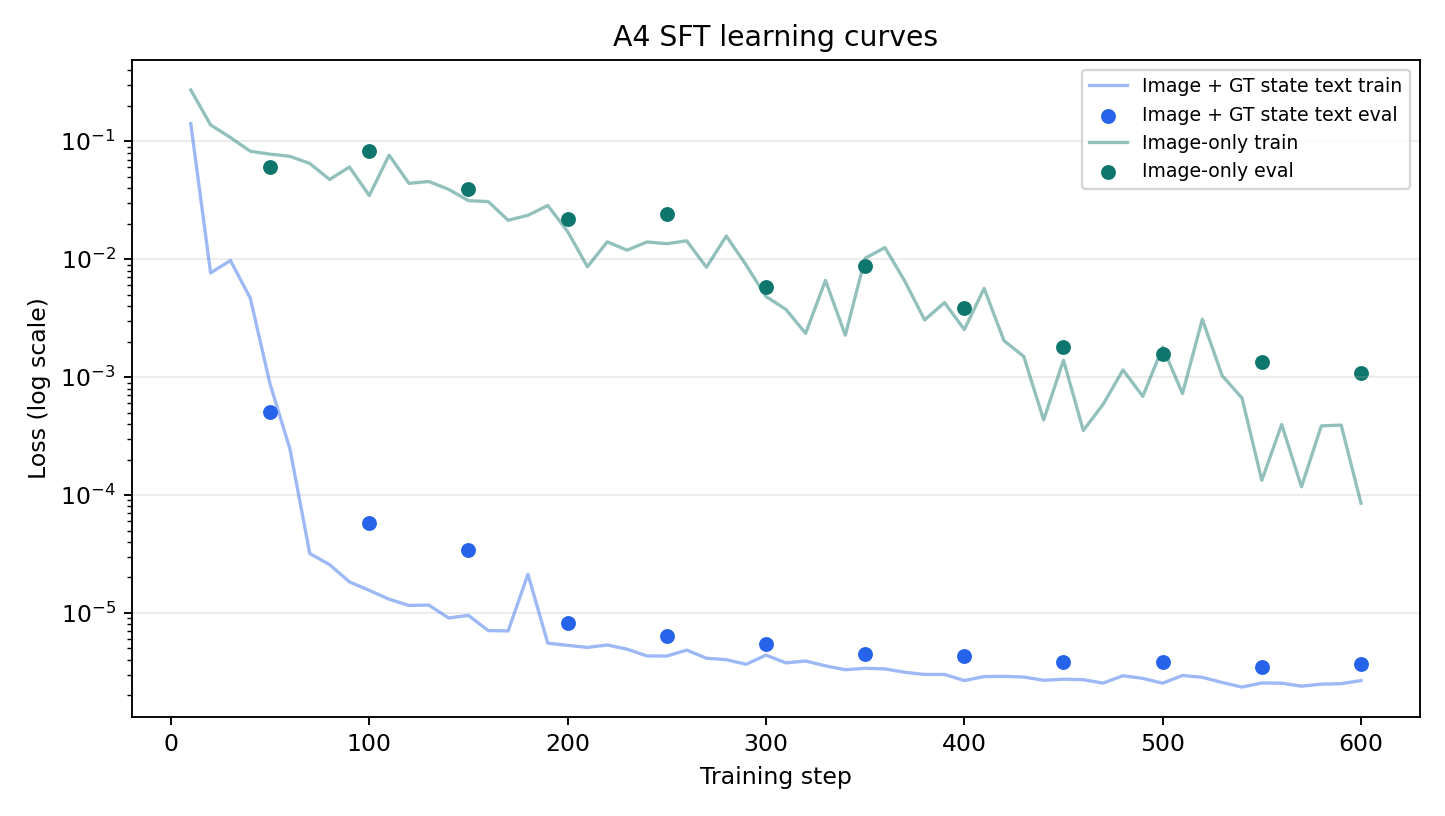
\includegraphics[width=\columnwidth]{assets/a4_learning_curve.png}
\caption{SFT learning curves.}
\label{fig:learning}
\end{figure}

\subsection{Calibration Gate}

Before trusting validation accuracy, I checked train accuracy. The rule was simple: if train both-correct accuracy (position and outcome both correct) is far below 90\%, do not interpret validation as meaningful.

Both models passed. SFT image + GT state text reached 1.0000 train both-correct; SFT image-only reached 0.9992. So the validation metrics are interpretable. This does not prove out-of-distribution generalization. It says the models fit the assignment distribution.

\subsection{One-Step Evaluation}

\begin{table*}[t]
\caption{Main one-step validation metrics. Both-correct means position and outcome are both correct.}
\label{tab:a5}
\centering
\scriptsize
\begin{tabular}{llrrrrrrrrr}
\toprule
Condition & Split & Count & Format & Exact & Pos. & Outcome & Both & Wrong pos. & Wrong out. & Format err. \\
\midrule
SFT image + GT state text & train & 2400 & 1.0000 & 1.0000 & 1.0000 & 1.0000 & 1.0000 & 0 & 0 & 0 \\
SFT image + GT state text & val & 600 & 1.0000 & 1.0000 & 1.0000 & 1.0000 & 1.0000 & 0 & 0 & 0 \\
SFT image-only & train & 2400 & 1.0000 & 0.9992 & 1.0000 & 0.9992 & 0.9992 & 0 & 2 & 0 \\
SFT image-only & val & 600 & 1.0000 & 0.9917 & 0.9950 & 0.9917 & 0.9917 & 3 & 5 & 0 \\
\bottomrule
\end{tabular}
\end{table*}

SFT image + GT state text was perfect on the measured train and validation splits. SFT image-only was still strong, but not perfect.

\begin{table}[t]
\caption{Validation outcome confusion, SFT image + GT state text. Rows are ground-truth outcomes; columns are predicted outcomes.}
\label{tab:conftext}
\centering
\small
\begin{tabular}{lrrrr}
\toprule
Target & Safe & Hole & Goal & Wall \\
\midrule
safe & 473 & 0 & 0 & 0 \\
hole & 0 & 29 & 0 & 0 \\
goal & 0 & 0 & 5 & 0 \\
wall & 0 & 0 & 0 & 93 \\
\bottomrule
\end{tabular}
\end{table}

\begin{table}[t]
\caption{Validation outcome confusion, SFT image-only. Rows are ground-truth outcomes; columns are predicted outcomes.}
\label{tab:confimage}
\centering
\small
\begin{tabular}{lrrrr}
\toprule
Target & Safe & Hole & Goal & Wall \\
\midrule
safe & 471 & 2 & 0 & 0 \\
hole & 2 & 27 & 0 & 0 \\
goal & 0 & 0 & 5 & 0 \\
wall & 1 & 0 & 0 & 92 \\
\bottomrule
\end{tabular}
\end{table}

The SFT image-only errors are small: safe vs hole, hole vs safe, and one wall case predicted as safe. I would not draw a strong perception conclusion from validation alone. The safer reading is narrower: image-only is slightly less perfect on this split, while SFT image + GT state text gives the model symbolic player, goal, and hole positions directly.

\subsection{Verdict}

Part 2 worked on the assignment's one-step generated-map distribution. GT state text helped, but the gap was small: 100.0\% both-correct for SFT image + GT state text versus 99.17\% for SFT image-only on validation.

The numbers are strong on the assignment distribution, but terminal outcomes are sparse: only 5 validation goal examples and 29 hole examples. I would not call this a broad solution to dynamics. The claim is narrower: it covers this fixed one-step task, map generator, and output format.

The more important lesson appears in Part 3. A one-step model can be very accurate offline and still be fragile inside a closed-loop planner.

\section{Part 3: Planning in Imagination}

\subsection{Hypothesis}

Before running the held-out planning comparison, I expected a clean ordering: GT one-step lookahead should be the ceiling, SFT image + GT state text should come next, SFT image-only should be lower because it has to read the board from pixels, and both zero-shot conditions should mostly fail at the strict output contract. I also expected the GT one-step-greedy ceiling to be fairly high, roughly 70--90\%, because the planner could reject immediate holes and walls. That last expectation was wrong.

\subsection{Design}

The planner is deliberately simple. For each real state: render the current image, ask the predictor for the next position and outcome for each action, reject predicted holes and walls, choose the remaining action closest to the GT goal by Manhattan distance, and execute that action in the real environment.

The predictor can be zero-shot Qwen, one of the SFT models, or GT transition logic. The VLM does not choose the action directly in lookahead conditions. It predicts one-step dynamics only.

For \code{lookahead\_sft\_image\_text}, each one-step query used the current rendered image plus GT state text recomputed from the real environment state. For \code{lookahead\_sft\_image\_only}, each query used the current rendered image and action only, with no GT state text.

All five planning-comparison conditions use the same held-out seeds, 100--129. These maps are separate from the training seeds 0--79 and validation seeds 80--99. For a fair comparison, the reactive baseline is rerun on the same held-out seed set.

\subsection{Results}

Metric denominators: success, hole, and truncation rates are per episode over 30 seeds. Mean steps is environment steps per episode. Format compliance and parse failure are per model output/query. Reactive uses one model query per environment step; lookahead uses four action queries per environment step. Fallback rate is per environment decision step.

For binary success and hole rates, I use Wilson 95\% intervals. The original bootstrap intervals were degenerate for some 0-count rates, which is misleading at $n=30$. Mean-step intervals remain bootstrap intervals.

\begin{table*}[t]
\caption{Main planning metrics on held-out seeds 100--129.}
\label{tab:a6main}
\centering
\scriptsize
\begin{tabular}{lrlrrrrr}
\toprule
Condition & Episodes & Successes & Success & Wilson 95\% CI & Mean steps & Hole & Trunc. \\
\midrule
reactive\_vlm & 30 & 0/30 & 0.0000 & [0.000, 0.114] & 22.50 & 0.8000 & 0.2000 \\
lookahead\_zeroshot\_vlm & 30 & 0/30 & 0.0000 & [0.000, 0.114] & 22.50 & 0.8000 & 0.2000 \\
lookahead\_sft\_image\_text & 30 & 5/30 & 0.1667 & [0.073, 0.336] & 59.03 & 0.3000 & 0.5333 \\
lookahead\_sft\_image\_only & 30 & 3/30 & 0.1000 & [0.035, 0.256] & 17.40 & 0.8000 & 0.1000 \\
lookahead\_gt & 30 & 6/30 & 0.2000 & [0.095, 0.373] & 82.80 & 0.0000 & 0.8000 \\
\bottomrule
\end{tabular}
\end{table*}

\begin{table}[t]
\caption{Interface diagnostics. Format and parse metrics are per model output/query; fallback is per environment decision.}
\label{tab:a6diag}
\centering
\scriptsize
\begin{tabular}{lrrrr}
\toprule
Condition & Format & Parse fail & Fallback & Runtime \\
\midrule
reactive\_vlm & 0.0000 & 1.0000 & 1.0000 & 156.3 \\
zeroshot\_lookahead & 0.0000 & 1.0000 & 1.0000 & 575.0 \\
sft\_image\_text & 1.0000 & 0.0000 & 0.0000 & 3813.3 \\
sft\_image\_only & 1.0000 & 0.0000 & 0.0000 & 1120.2 \\
lookahead\_gt & 1.0000 & 0.0000 & 0.0000 & 6.8 \\
\bottomrule
\end{tabular}
\end{table}

\begin{figure*}[t]
\centering
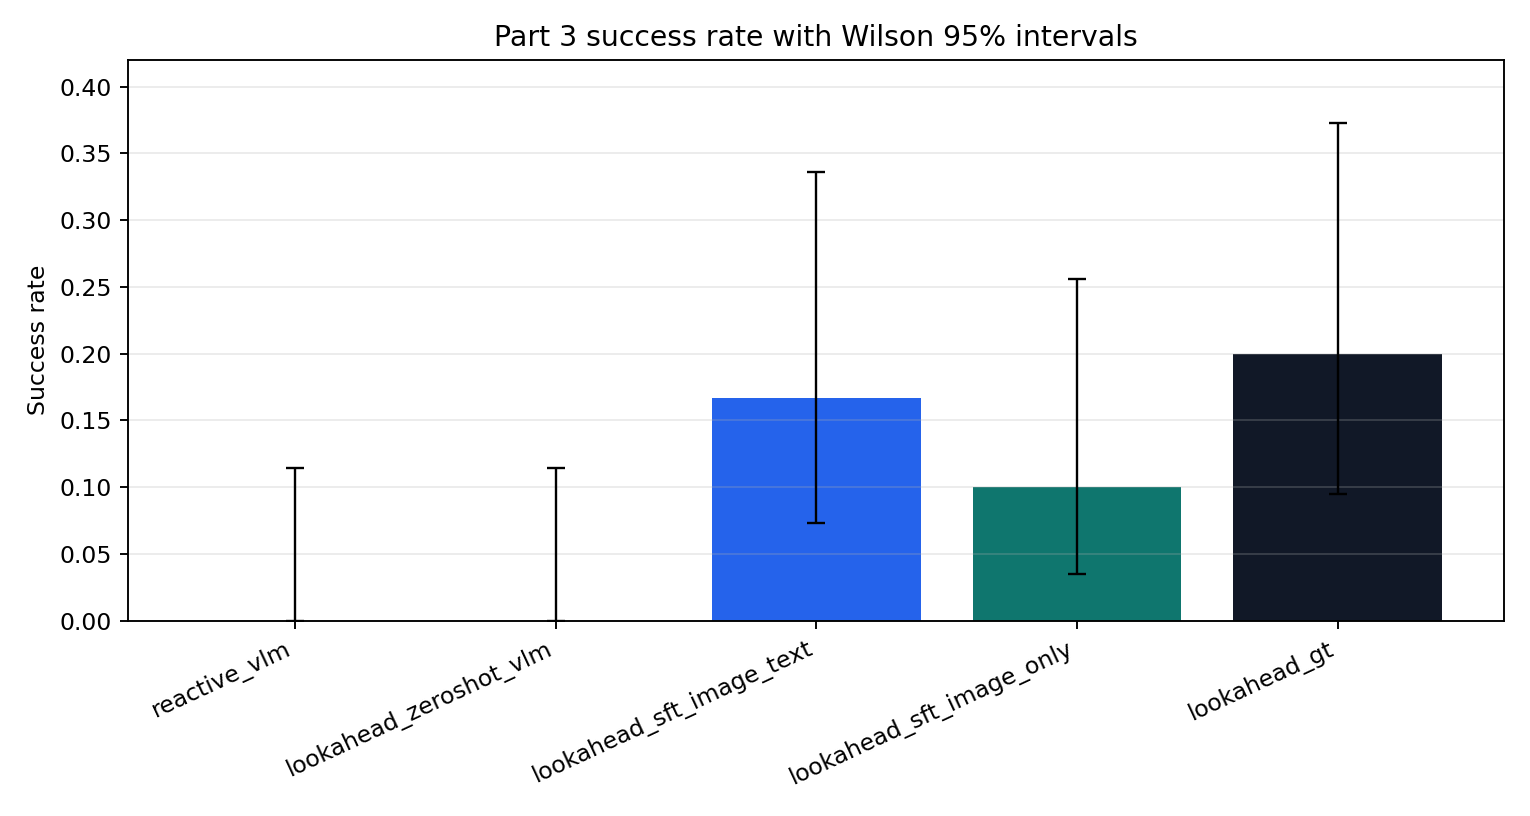
\includegraphics[width=0.72\textwidth]{assets/part3_success_rate_wilson_ci.png}
\caption{Part 3 success rates with Wilson confidence intervals. At $n=30$, the intervals are wide.}
\label{fig:a6success}
\end{figure*}

The ordering roughly matches the hypothesis, but the ceiling is much lower than I expected. SFT image + GT state text is the best observed learned condition at 16.7\% success, or 5/30 maps. SFT image-only reaches 10.0\%, or 3/30. The GT one-step-greedy planner reaches 20.0\%, or 6/30. With 30 seeds, the confidence intervals are wide, so I would not claim a clean statistical separation between the learned conditions. The failure modes matter more than the small ranking.

\subsection{What Went Wrong}

Zero-shot failed at the interface again. Reactive Qwen returned strings like \code{Down}. Zero-shot world-model Qwen returned strings like:

\begin{verbatim}
Position: (0, 1). Outcome: safe
\end{verbatim}

Both are close to useful. Both are invalid under the strict parser. The measured strict-format compliance is 0.0000 for both zero-shot conditions. I keep that as the assignment metric, then separate it from semantic intent with a relaxed manual-parser diagnostic for the reactive outputs.

A human or LLM-based parser can read \code{Down}. The strict parser cannot accept it under the declared contract. I therefore added the relaxed always-Down diagnostic in Table~\ref{tab:downrelaxed}: even if \code{Down} is accepted as an action, it still solves 0/30 maps on both seed sets.

The SFT models fixed the format contract. Both SFT planning conditions had format compliance 1.0000 and parse failure 0.0000. After that, the important closed-loop questions are prediction quality and planning.

Closed-loop prediction diagnostics are less clean than iid validation metrics, but they are useful. I recomputed the true deterministic transition for every saved lookahead query and compared it with the model prediction in the trace.

\begin{table}[t]
\caption{Closed-loop prediction diagnostics from saved planning traces.}
\label{tab:closedloop}
\centering
\scriptsize
\begin{tabular}{lrrrr}
\toprule
Condition & All correct & All total & Sel. correct & Sel. total \\
\midrule
sft\_image\_text & 6368 & 7084 & 1124 & 1771 \\
sft\_image\_only & 1981 & 2088 & 497 & 522 \\
\bottomrule
\end{tabular}
\end{table}

The selected-action accuracies are 0.6347 for SFT image + GT state text and 0.9521 for SFT image-only. This is a diagnostic, not the headline. These are closed-loop visited-state distributions, not iid validation rows. The inversion does not mean SFT image-only is the better world model: SFT image + GT state text ran about 3.4$\times$ longer by mean episode length, so it accumulated many repeated-loop queries outside the training distribution. Direct comparison is messy. Possible explanations include on-policy distribution shift, repeated-state artifacts, prompt/context mismatch, the planner selecting actions where mistakes matter most, and limits of this trace-labeling diagnostic. The useful point is smaller: offline one-step validation accuracy did not transfer cleanly to every state visited by the planner.

The safety-critical errors are more revealing than aggregate both-correct accuracy. A false-safe prediction means the model says an action is usable, while the true transition is a \code{hole} or \code{wall}. A filter-based planner cannot recover from those if it selects the action.

\begin{table*}[t]
\caption{Safety-critical closed-loop errors. False-safe true-hole errors are the fatal ones.}
\label{tab:safety}
\centering
\scriptsize
\begin{tabular}{lrrrrrr}
\toprule
Condition & Sel. false-safe hole & Sel. false-safe wall & All false-safe hole & All false-safe wall & False-reject safe & Hole final false-safe \\
\midrule
lookahead\_sft\_image\_text & 9 & 638 & 16 & 700 & 0 & 9/9 \\
lookahead\_sft\_image\_only & 24 & 1 & 46 & 45 & 8 & 24/24 \\
\bottomrule
\end{tabular}
\end{table*}

For SFT image + GT state text, every hole episode ended with a selected false-safe action: 8 final steps predicted \code{goal} but were truly \code{hole}, and 1 predicted \code{safe} but was truly \code{hole}. For SFT image-only, all 24 hole episodes ended with final predictions of \code{safe} for true holes. Truncations are different: SFT image + GT state text had 9 truncation episodes with no selected model error and 7 with selected model errors; SFT image-only had 3 truncations, all with no selected model error.

The GT condition exposes the planning problem. It never steps into a hole, so its 0.0000 hole rate is reassuring. But it truncates on 80.0\% of maps. Seed 100 is a representative failure: perfect one-step predictions, 100 steps, no goal. The planner can avoid immediate danger but still fail to make progress.

This was not because the held-out maps were impossible. As a CPU-only diagnostic, I ran BFS over non-hole cells for seeds 100--129. All 30 maps were reachable, all had shortest paths within the 100-step cap, the mean shortest path was 14.13 steps, and the maximum was 16. The low GT result is about the GT one-step-greedy planner, not map impossibility.

\begin{table}[t]
\caption{Seed 100 GT one-step-greedy loop.}
\label{tab:loop}
\centering
\small
\begin{tabular}{rlll}
\toprule
Step & Position & Action & Next position \\
\midrule
9 & (2, 7) & Left & (2, 6) \\
10 & (2, 6) & Right & (2, 7) \\
11 & (2, 7) & Left & (2, 6) \\
\bottomrule
\end{tabular}
\end{table}

This is the key negative result. Moving planning out of the VLM does not make planning good by itself. The external planner still has to be a good planner.

\section{What Actually Bottlenecked?}

Two main issues show up in the experiments.

\textbf{First: output formatting.} Zero-shot Qwen gave near-miss strings rather than the required tags. I report that as a formatting violation under the strict contract, not as evidence that Qwen cannot choose an action. The relaxed manual-parser check keeps those two questions separate: accepting \code{Down} as an action still gives an always-Down policy with 0/30 successes.

\textbf{Second: one-step greedy planning.} GT dynamics shows that one-step greedy planning has a low ceiling; learned-model planning is limited by both on-policy prediction errors and planner myopia. Perfect one-step GT predictions only reached 20.0\% success. The planner is greedy, has no memory, and does not search over routes. It optimizes the next predicted Manhattan distance, not the path.

The model learned the local physics. The planner did not learn a global strategy. I mean that in the narrow sense supported here: offline validation showed strong one-step prediction on the assignment distribution, while the GT one-step-greedy ceiling and closed-loop traces showed that local predictions were not enough for reliable route-finding.

\section{Limitations and Future Work}

This is a homework report, not a broad benchmark. The limitations are concrete. Part 3 uses 30 maps, so the confidence intervals are wide. Train and validation maps come from the same generator distribution. The relaxed always-Down check is only a diagnostic for semantic intent; it is not the strict assignment metric. The planner is only one-step greedy. It has no visited-state penalty, no graph search, no value function, and no uncertainty handling.

I also did not implement the bonus experiments: no H=2/H=3 lookahead, no CoT planning, no 4$\times$4 comparison. No bonus experiments (A, B, or C) were attempted.

The obvious next step is not ``train harder.'' The one-step validation metrics are already high. Better diagnostics would be richer relaxed-parser zero-shot evaluation, H=2 or H=3 lookahead, a visited-state penalty or BFS-style planner using the learned model, uncertainty calibration for unsafe predictions, and a 4$\times$4 vs 8$\times$8 comparison to separate map scale from model quality.

\section{Conclusion}

The answer is split.

Yes, a VLM can learn to imagine one-step FrozenLake transitions on this same generated-map distribution and fixed post-SFT output format. In this setup, supervised Qwen2.5-VL adapters reached 100.0\% validation both-correct accuracy for SFT image + GT state text and 99.17\% for SFT image-only.

No, that did not make the planner strong. The best observed learned planning condition reached 16.7\% success, and the perfect GT one-step-greedy planner reached only 20.0\%. That ceiling changes how I read the rest of the results.

The blunt version is: on this one-step task, the model learned the physics; the planner still got lost.

\section*{Reproducibility Notes}

Main scripts are \path{run_a2_reactive_vlm.py}, \path{collect_data.py}, \path{train_sft.py}, \path{eval_world_model.py}, \path{run_planning.py}, and \path{plot_results.py}. Main source artifacts include the final metric tables, confusion matrices, planning traces, summaries, and derived plots under \path{results/}.

\end{document}
